
\phantom{There is some latex bug somewhere and this dummy call is needed to force it to make pdf...}



\begin{figure*}[ht]
  \centering
  \includegraphics[width=18cm]{lc_pair.png}
  \vskip -0.5in
  \caption{An example of a Blazhko star (LINEARid = 1212611) with LINEAR (top row) and ZTF (bottom row) light
    curves (left panels, data points with ``error bars''), phased light curves normalized to the 0--1 range (right panels, data points
    with ``error bars''), with their best-fit models shown by dashed lines. The best-fit period is determined for each
    dataset separately using 3 Fourier terms. The models shown in the right panels are evaluated with 6 Fourier terms. }
 \label{fig:lc_pair}
\end{figure*}


\section{Data Description and Period Estimation \label{sec:data}}

Analysis of field RR Lyrae stars requires a sensitive time-domain photometric survey over a large sky area.
For our starting sample, we used $\sim$3,000 field RR Lyrae stars with light curves obtained by the LINEAR
asteroid survey. In order to study long-term changes in light curves, we also utilized light curves obtained
by the ZTF survey which monitored the sky $\sim$15 years after LINEAR. The combination of LINEAR and
ZTF provided a unique opportunity to systematically search for the Blazhko effect in a large number of
field RR Lyrae stars.


We first describe each dataset in more detail, and then introduce our analysis methods. All our analysis
code, written in Python, is available on GitHub\footnote{\url{https://github.com/emadonev/var_stars}}.  
 
\subsection{LINEAR Dataset}

The properties of the LINEAR asteroid survey and its photometric re-calibration based on SDSS data are discussed
in \cite{2011AJ....142..190S}. Briefly, the LINEAR survey covered about 10,000 deg$^2$ of the northern sky in white
light (no filters were used, see Figure 1 in \citealt{2011AJ....142..190S}), with photometric errors ranging from $\sim$0.03
mag at an equivalent SDSS magnitude of $r=15$ to 0.20 mag at $r\sim18$. Light curves used in this work include,
on average, 270 data points collected between December 2002 and September 2008.
 
A sample of 7,010 periodic variable stars with $r<17$ discovered in LINEAR data were robustly classified by
\cite{2013AJ....146..101P}, including
about $\sim$3,000 field RR Lyrae stars of both ab and c type, detected to distances of about 30 kpc \citep{2013AJ....146...21S}.
The sample used in this work contains 2196 ab-type and 745 c-type RR Lyrae, selected using classification labels and the {\it gi}
color index from \cite{2013AJ....146..101P}.
The LINEAR light curves, augmented with IDs, equatorial coordinates, and other data, were accessed using the astroML Python
module\footnote{For an example of light curves, see \url{https://www.astroml.org/book_figures/chapter10/fig_LINEAR_LS.html}}
\citep{2012cidu.conf...47V}. 


\subsection{ZTF Dataset}

The Zwicky Transient Factory (ZTF) is an optical time-domain survey that uses the Palomar 48-inch Schmidt telescope
and a camera with 47 deg$^2$ field of view \citep{2019PASP..131a8002B}. The dataset analyzed here was obtained with
SDSS-like $g$, $r$, and $i$ band filters. Light curves for objects in common with the LINEAR RR Lyrae sample typically
have smaller random photometric errors than LINEAR light curves because ZTF data are deeper (compared to LINEAR,
ZTF data have about 2-3 magnitudes fainter  $5\sigma$ depth). ZTF data used in this work were collected between
February 2018 and December 2023, on average about 15 years after obtaining LINEAR data. 

The ZTF dataset for this project was created by selecting ZTF IDs with matching equatorial coordinates to a corresponding
LINEAR ID of an RR Lyrae star. This process used the {\it ztfquery} function, which searched the coordinates in the ZTF database
within 3 arcsec from the LINEAR position. The resulting sample consisted of 2857 RR Lyrae stars with both LINEAR and ZTF data.
The fractions of RRab and RRc type RR Lyrae in this sample, 71\% RRab and 29\% RRc type, are consistent with results from
other surveys \citep[e.g.,][]{2010ApJ...708..717S}. 


\subsection{Period Estimation}


The first step of our analysis is estimating best-fit periods, separately for LINEAR and ZTF datasets. 
We used the Lomb-Scargle method \citep{2015zndo.....14833V} as implemented in {\it astropy}
\citep{2018AJ....156..123A}. The period estimation used 3 Fourier components and a two-step process: an initial
best-fit frequency was determined using the {\it autopower} frequency grid option and then the power spectrum was
recomputed around the initial frequency using an order of magnitude smaller frequency step. In case of ZTF, we
estimated period separately for each available passband and adopted their mean value. Once the best-fit
period was determined, a best-fit model for the phased light curve was computed using 6 Fourier components.
Fig \ref{fig:lc_pair} shows an example of a star with LINEAR and ZTF light curves, phased light curves, and their
best-fit models.  

We found excellent agreement between the best-fit periods estimated separately from LINEAR and ZTF light curves. 
The median of their ratio is unity within $2\times10^{-6}$ and the robust standard deviation of their ratio is
$2\times10^{-5}$. With a median sample period of 0.56 days, the implied scatter of period difference is about 1.0 sec.  

Given on average about 15 years between LINEAR and ZTF data sets, and a typical period of 0.56 days, this time
difference corresponds to about 10,000 oscillations. With a fractional period uncertainty of $2\times10^{-5}$,
LINEAR data can predict the phase of ZTF light curve with an uncertainty of 0.2. Therefore, for a robust detection
of light curve phase modulation, each data set must be analyzed separately. On the other hand, amplitude
modulation can be detected on time scales as long as 15 years, as discussed in the following section. 



\section{Analysis Methodology: Searching for the Blazhko Effect  \label{sec:analysis}}  

\begin{figure}[ht]
\resizebox{\hsize}{!}{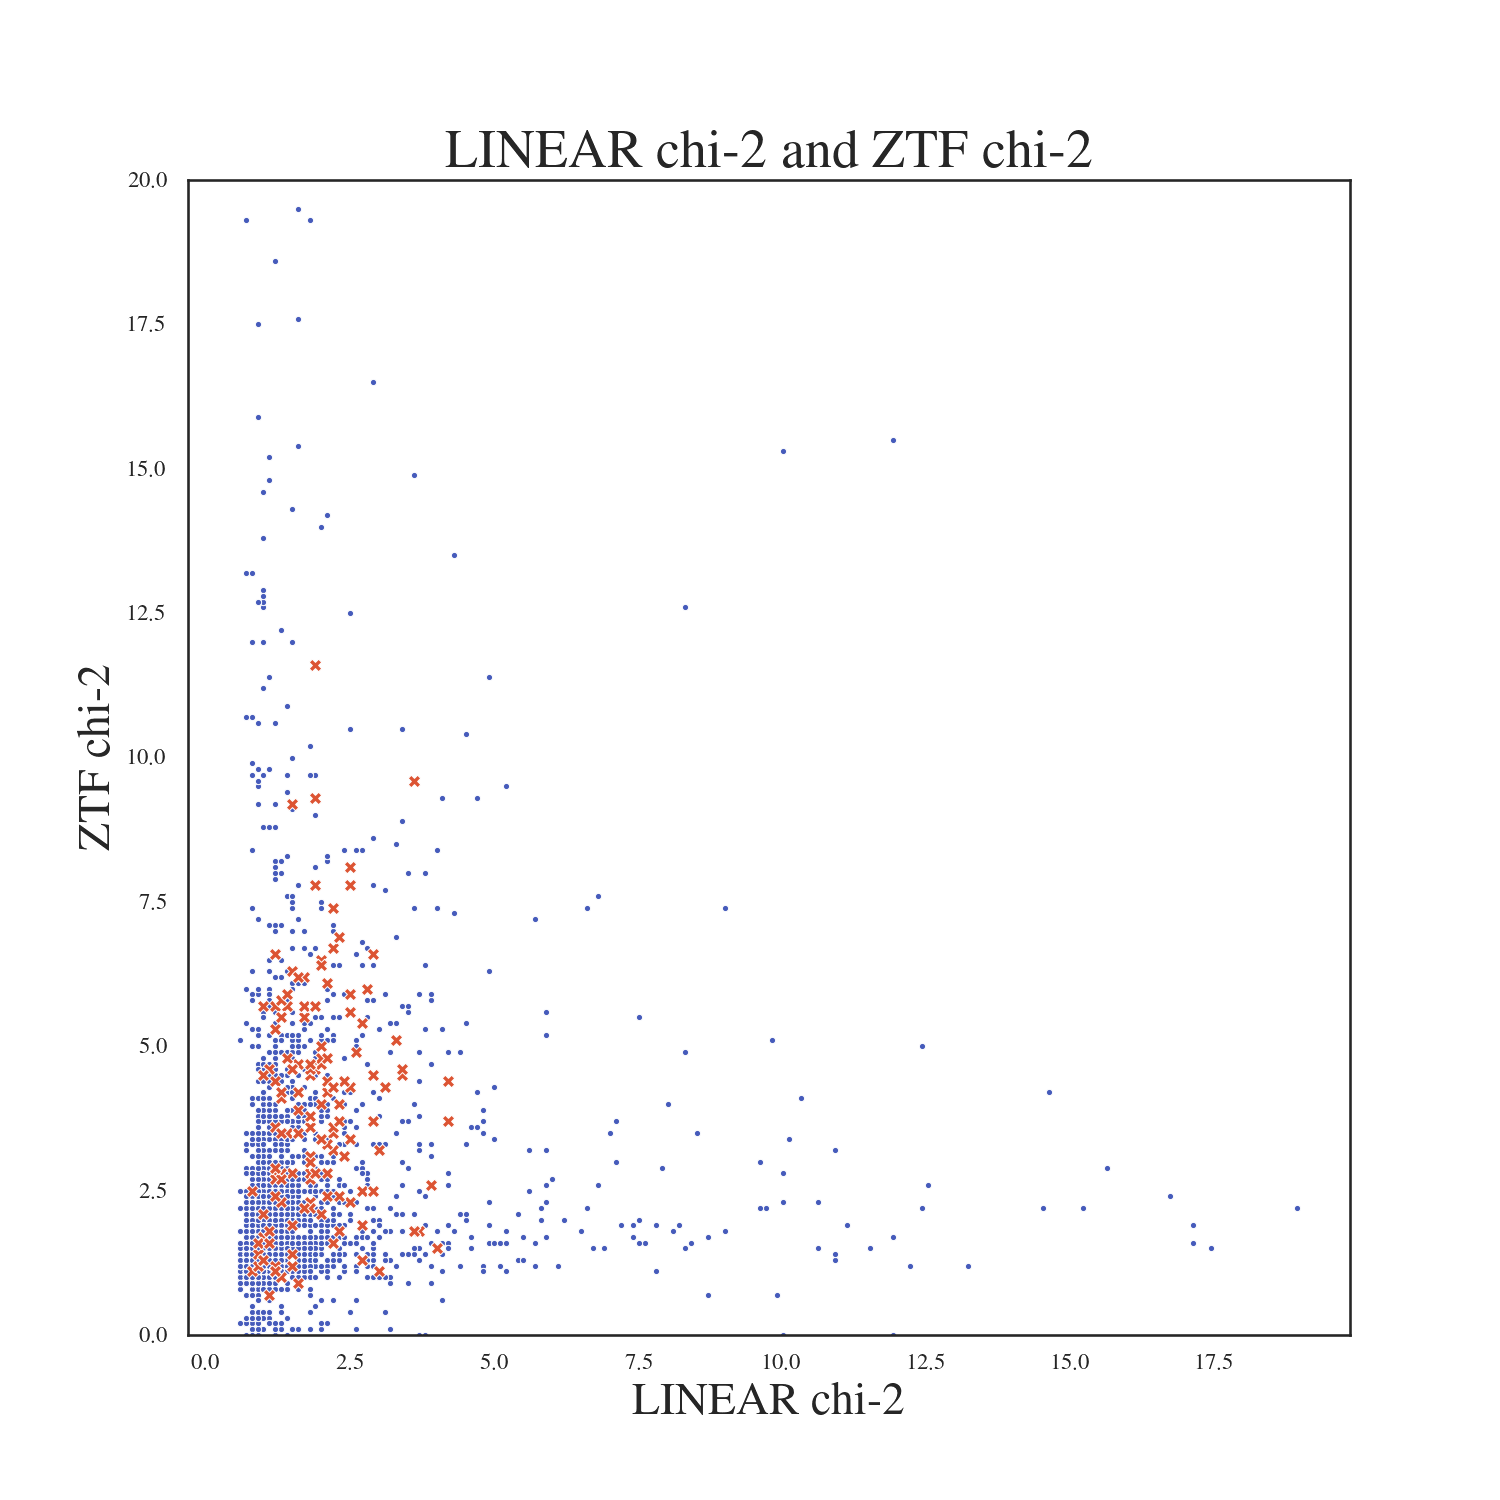
\includegraphics[width=17cm]{chi_scatter.png}}
\caption{A selection diagram constructed with the two sets of robust $\chi^2_{dof}$ values, for LINEAR and ZTF data sets, where
  blue symbols represents all RR Lyrae stars and the red symbols are the final sample of Blazhko stars. The horizontal
  and vertical dashed lines mark Blazhko candidate selection boundaries (see text).}
\label{fig:chi2}
\end{figure}


Given the two sets of light curves from LINEAR and ZTF, we searched for amplitude and phase modulation,
either during the 5-6 years of data taking by each survey, or during the average span of 15 years between the two
surveys. Starting with a sample of 2857 RR Lyrae stars, we pre-selected a smaller sample that was inspected
visually (see below for details). We also required at least 250 LINEAR data points and 40 ZTF data points (per band)
in analyzed light curves. We used two pre-selection methods that are sensitive to different types of light curve
modulation: direct light curve analysis and periodogram analysis, as follows.
 

 
\subsection{Direct Light Curve Analysis}

\begin{figure*}[ht]
    \centering
    \resizebox{\hsize}{!}{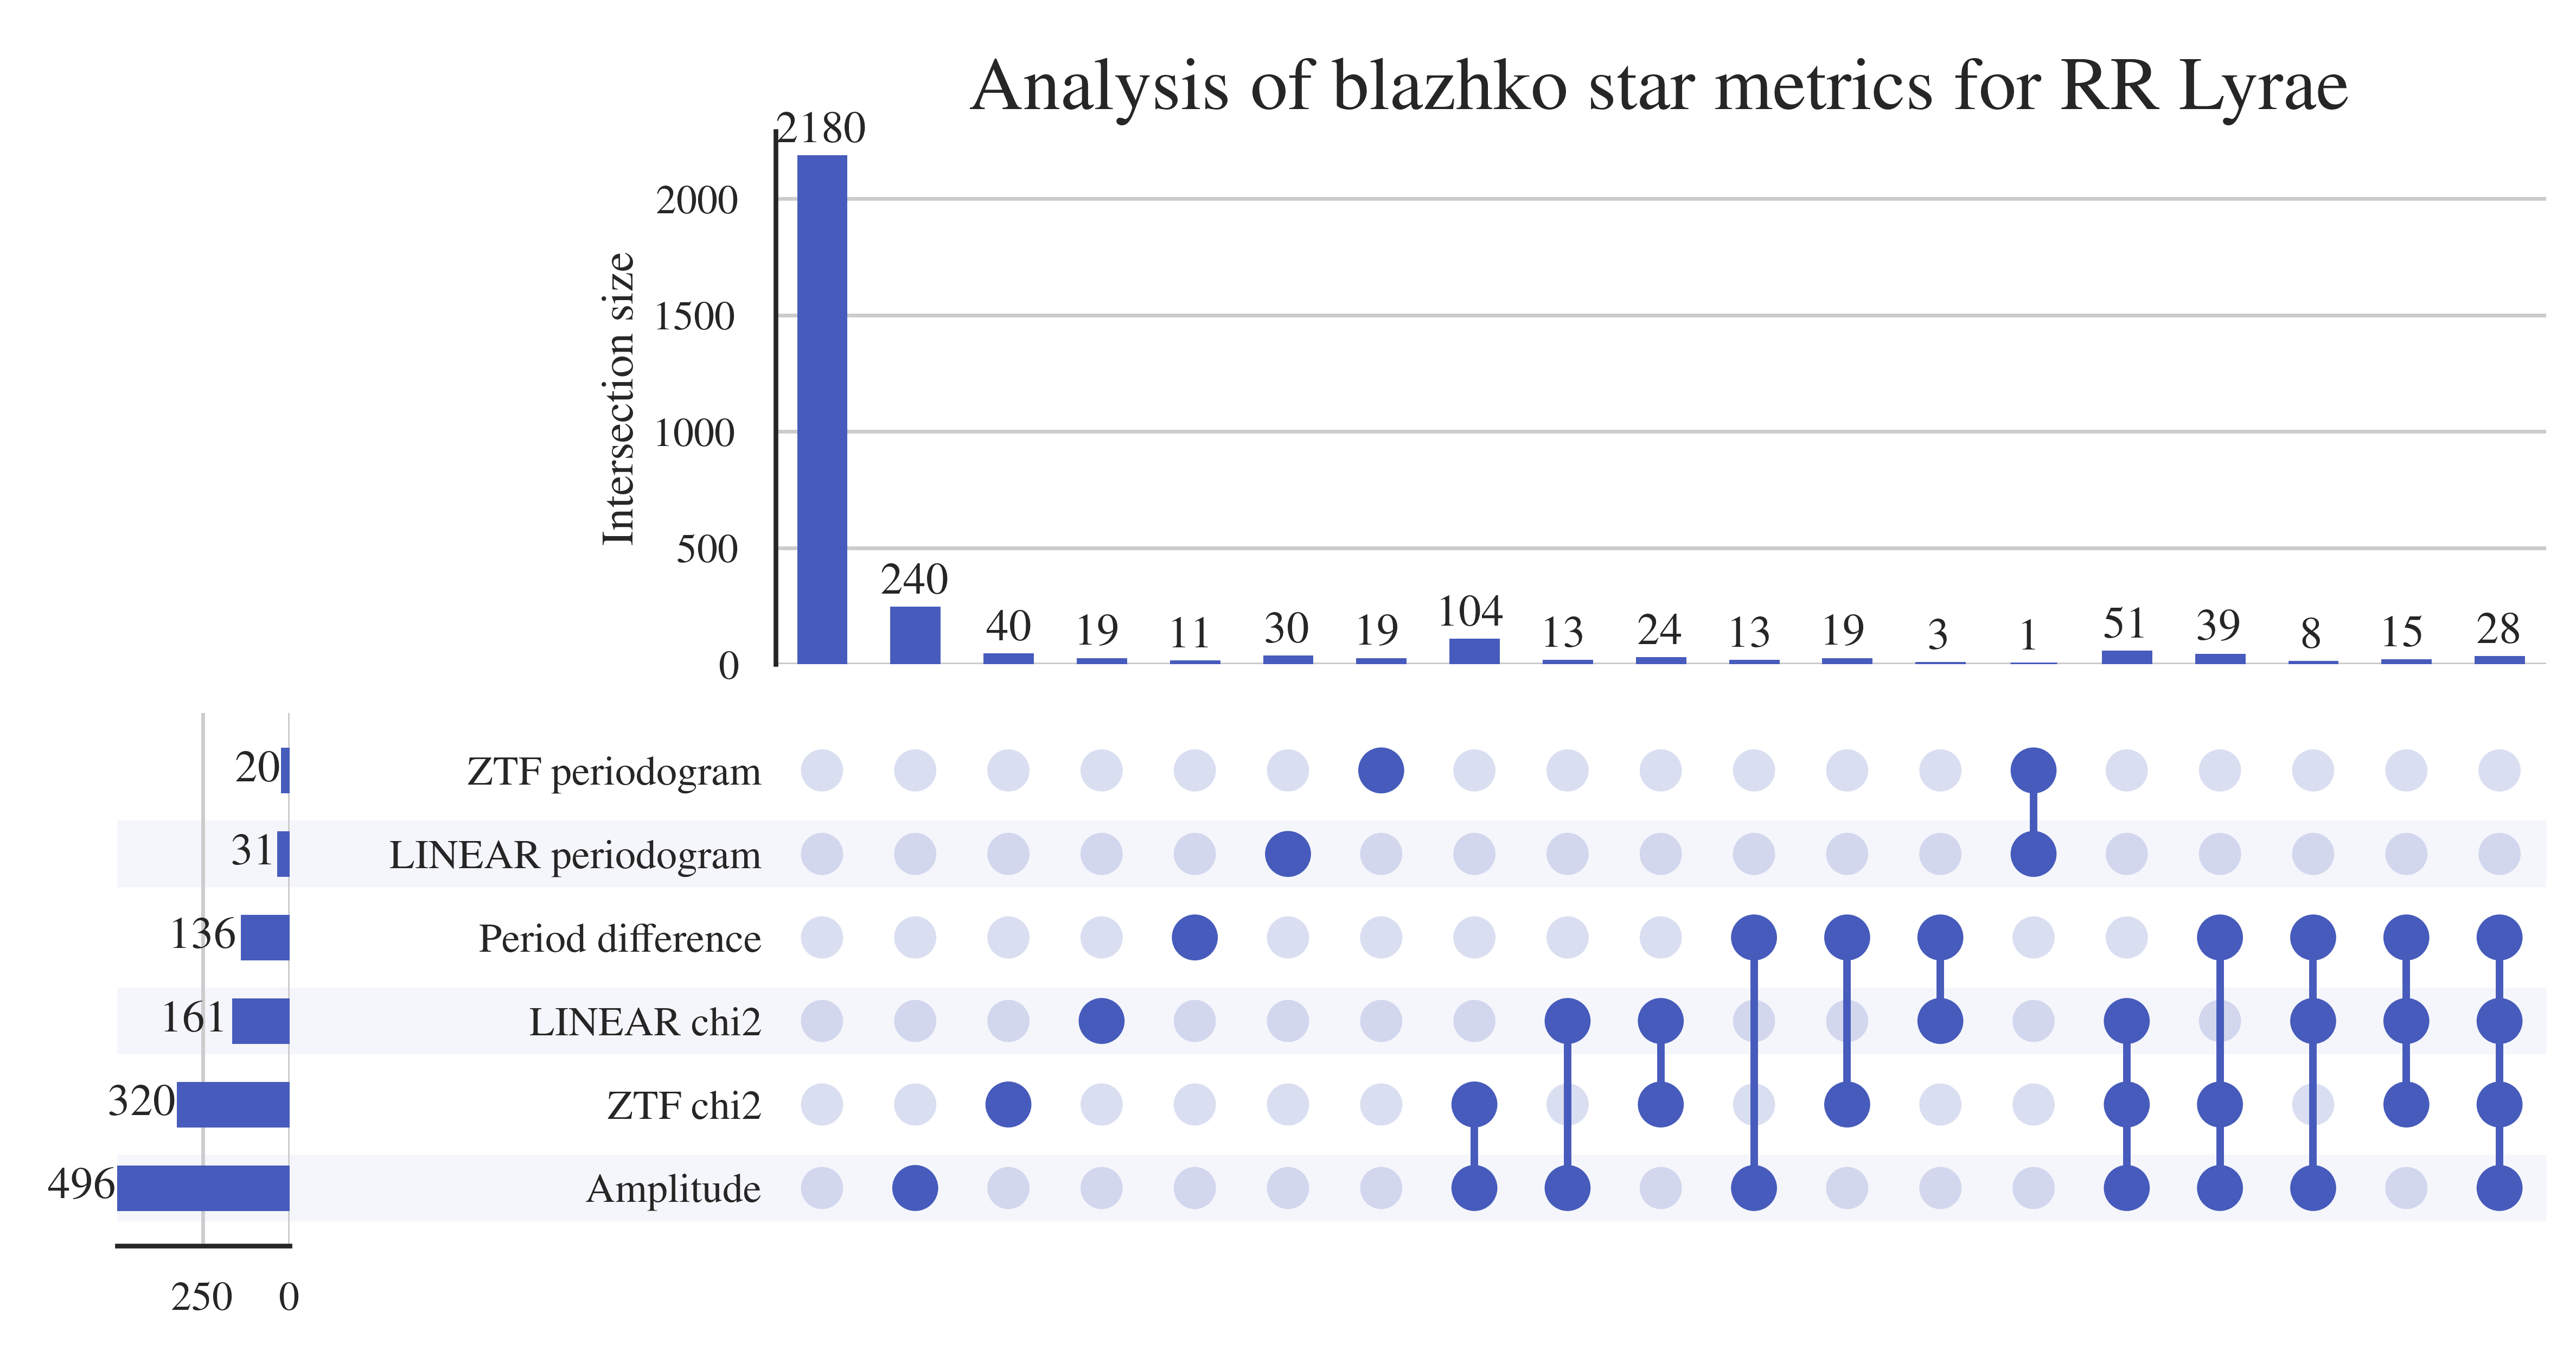
\includegraphics[width=22cm]{stats_categories.png}}
    \vskip -0.3in
    \caption{The figure shows selection criteria and the resulting numbers of pre-selected Blazhko star candidates for each
      criterion and their combinations. The dots represent each case a star can occupy, where every solid dot is a specific
      criterion that is satisfied. Connections between solid dots represent stars which satisfy multiple criteria. Each dot
      combination has its own count, represented by the horizontal countplot. The vertical countplot shows the total number
      of stars that satisfy one criteria (union of all cases).}
      \label{fig:selstats}
    \end{figure*}
    
Given statistically correct period, amplitude and light curve shape estimates,
as well as data being consistent with reported (presumably Gaussian) uncertainty estimates, the $\chi^2$ per degree
of freedom gives a quantitative assessment of the \textit{"goodness of fit"},
\begin{equation}
        \chi_{dof}^2 = {1 \over N_{dof}} \, \sum{\frac{(d_i - m_i)^2}{\sigma_i^2}}.
\end{equation}
Here, $d_i$ are measured light curve data values at times $t_i$, and with associated uncertainties $\sigma_i$,
$m_i$ are best-fit models at times $t_i$, and $N_{dof}$ is the number of degrees of freedom, essentially the
number of data points. In the absence of any light curve modulation, the expected value of $\chi^2_{dof}$ is
unity, with a standard deviation of $\sqrt(2/N_{dof}$.  If $\chi^2_{dof} - 1$ is many times  larger than 
$\sqrt(2/N_{dof}$, it is unlikely that data $d_i$ were generated by the assumed (unchanging) model $m_i$.  
Of course, $\chi^2_{dof}$ can also be large due to underestimated measurement uncertainties $\sigma_i$,
or to occasional non-Gaussian measurement error (the so-called outliers). 

Therefore, to search for signatures of the Blazhko effect, manifested through statistically unlikely large values
of $\chi^2_{dof}$, we computed $\chi^2_{dof}$ separately for LINEAR and ZTF data (see Figure~\ref{fig:chi2}). 
Using the two sets of $\chi^2_{dof}$ values, we algorithmically pre-selected a sample of candidate Blazhko stars
for further visual analysis of their light curves. The visual analysis is needed to confirm the expected Blazhko behavior
in observed light curves, as well as to identify cases of data problems, such as photometric outliers. 

We used a simple scoring algorithm, optimized through trial and error,
such that for LINEAR the range $1.8<\chi^2_{dof}<3.0$ was worth 2 points and $\chi^2_{dof}>3.0$ worth 3 points,
while for ZTF $2.0<\chi^2_{dof}<4.0$ and $\chi^2>4.0$ were the analogous limits. In addition, we also considered
normalized period differences ($dP$ and amplitude differences ($dA$) and assigned: 2 points for $0.00002 < dP < 0.00005$
and 4 points for $dP > 0.00005$; 1 point for $0.05 < dA < 0.15$ and 2 points for $dA > 0.15$. 
A star could score a maximum of 12 points, and a minimum of 5 points was required for further visual analysis. 

The sample pre-selected using this method includes 189 stars. For most selected stars, the $\chi^2_{dof}$ values were
larger for the ZTF data because the ZTF photometric uncertainties are smaller than for the LINEAR data set. 
Fig.~\ref{fig:selstats} summarizes the selection criteria and the resulting numbers of selected stars for each
criterion and their combinations. 
 


\subsection{Periodogram Analysis} 


\begin{figure*}[ht]
  \centering
  \resizebox{\hsize}{!}{\includegraphics[width=14cm]{periodogram.png}}
  \caption{The top two panels show a simulated periodogram for a sum of two {\it sine} functions with similar frequencies
    $f_1$ and  $f_2$ --   the central peak corresponds to their mean (see eqs.~\ref{eq:fo} and \ref{eq:Df}).
    The bottom left panel shows a periodogram for an observed LINEAR light curve, and the bottom right panel shows its
    folded version (around the main frequency $f_o=1.585$ d$^{-1}$). In the bottom left panel, the three vertical dashed
    lines show the three  frequencies identified by the algorithm described in text, and the two dot-dashed lines mark
    yearly aliases around the main frequency $f_o$, at frequencies $f_o \pm 0.00274$ d$^{-1}$. The two vertical lines in the
    bottom right panel have the same meaning, and the horizontal dashed line shows the noise level multiplied by 5.}
\label{fig:periodogram}
\end{figure*}

  
When light curve modulation is due to double-mode oscillation with two similar oscillation frequencies (periods),
it is possible to recognize its signature in the periodogram computed as part of the Lomb-Scargle analysis. Depending
on various details, such as data sampling and the exact values of periods, amplitudes, this method may be
more efficient than direct light curve analysis \citep{2020MNRAS.494.1237S}. 

A sum of two {\it sine} functions with same amplitudes and with frequencies $f_1$ and $f_2$ can be rewritten 
using trigonometric equalities as 
\begin{equation}
         y(t) = 2 \, \cos(2\pi{f_1-f_2\over 2} t) \, \sin(2\pi {f_1+f_2\over 2} t).
\end{equation} 
We can define 
\begin{equation}
\label{eq:fo}
         f_o = {f_1+f_2\over 2},
\end{equation} 
and 
\begin{equation}
\label{eq:Df}
         \Delta f = |{f_1-f_2\over 2}|,
\end{equation} 
with $\Delta f << f_o$ when $f_1$ and $f_2$ are similar. The fact that $\Delta f$ is much smaller than $f_o$ means
that the period of the {\it cos} term
is much larger than the period of the basic oscillation ($f_o$). In other words, the {\it cos} term acts as a slow
amplitude modulation of the basic oscillation. When the amplitudes of two {\it sine} functions are not equal, the
results are more complicated but the basic conclusion about amplitude modulation remains.
When the power spectrum of $y(t)$ is constructed, it will show 3 peaks: the main peak at $f_o$ and
two more peaks at frequencies $f_o \pm \Delta f$. We used this fact to construct an algorithm for
automated searching for the evidence of amplitude  modulation. 
Fig \ref{fig:periodogram} compares the theoretical periodogram produced by interference beats with our algorithm's periodogram,
signifying that local Blazhko peaks are present in real data.


After the strongest peak in the Lomb-Scargle periodogram is found at frequency $f_o$, we search for  two equally
distant local peaks at frequencies $f_-$ and $f_+$, with $f_- < f_0 < f_+$.  The sideband peaks can be highly asymmetric
\cite{2003ApJ...598..597A} and observed periodograms can sometimes be much more complex \cite{2007MNRAS.377.1263S}.  
We fold the periodogram through the main peak at $f_o$, multiply the two branches and then search for the strongest peaks
in the resulting folded periodogram that is statistically more significant than the background noise. The background noise
is computed as the scatter of the folded periodogram estimated from the interquartile range. We require a ``signal-to-noise''
ratio of at least 5, as well as the peak strength of at least 0.05. 
If such a peak is found,
and it doesn't correspond to yearly alias, we select the star as a candidate Blazhko star and compute
its Blazhko period as 
\begin{equation*}
P_{BL} = |f_{-,+} - f_0|^{-1},
\end{equation*}
where $f_{-,+}$ means the Blazhko sideband frequency with a higher amplitude is chosen. 

The observed Blazhko periods range from 3 to 3,000 days, and Blazhko amplitudes range from 0.01 mag to about 0.3 mag \citep{2007MNRAS.377.1263S}. In this work, we selected a smaller Blazhko range due to the limitations of our data: 30--325 days. 
With this additional constraint, we selected 51 candidate Blazhko stars, with one star already included in the sample
of 189 stars described in preceding section. 
Fig \ref{fig:phase2} shows an example where two very prominent peaks were identified in the LINEAR periodogram. 



\subsubsection{Visual Confirmation}

\begin{figure*}[ht]
  \centering
%  
\includegraphics[width=17cm]{LCplot_7048826.png}
  \resizebox{\hsize}{!}{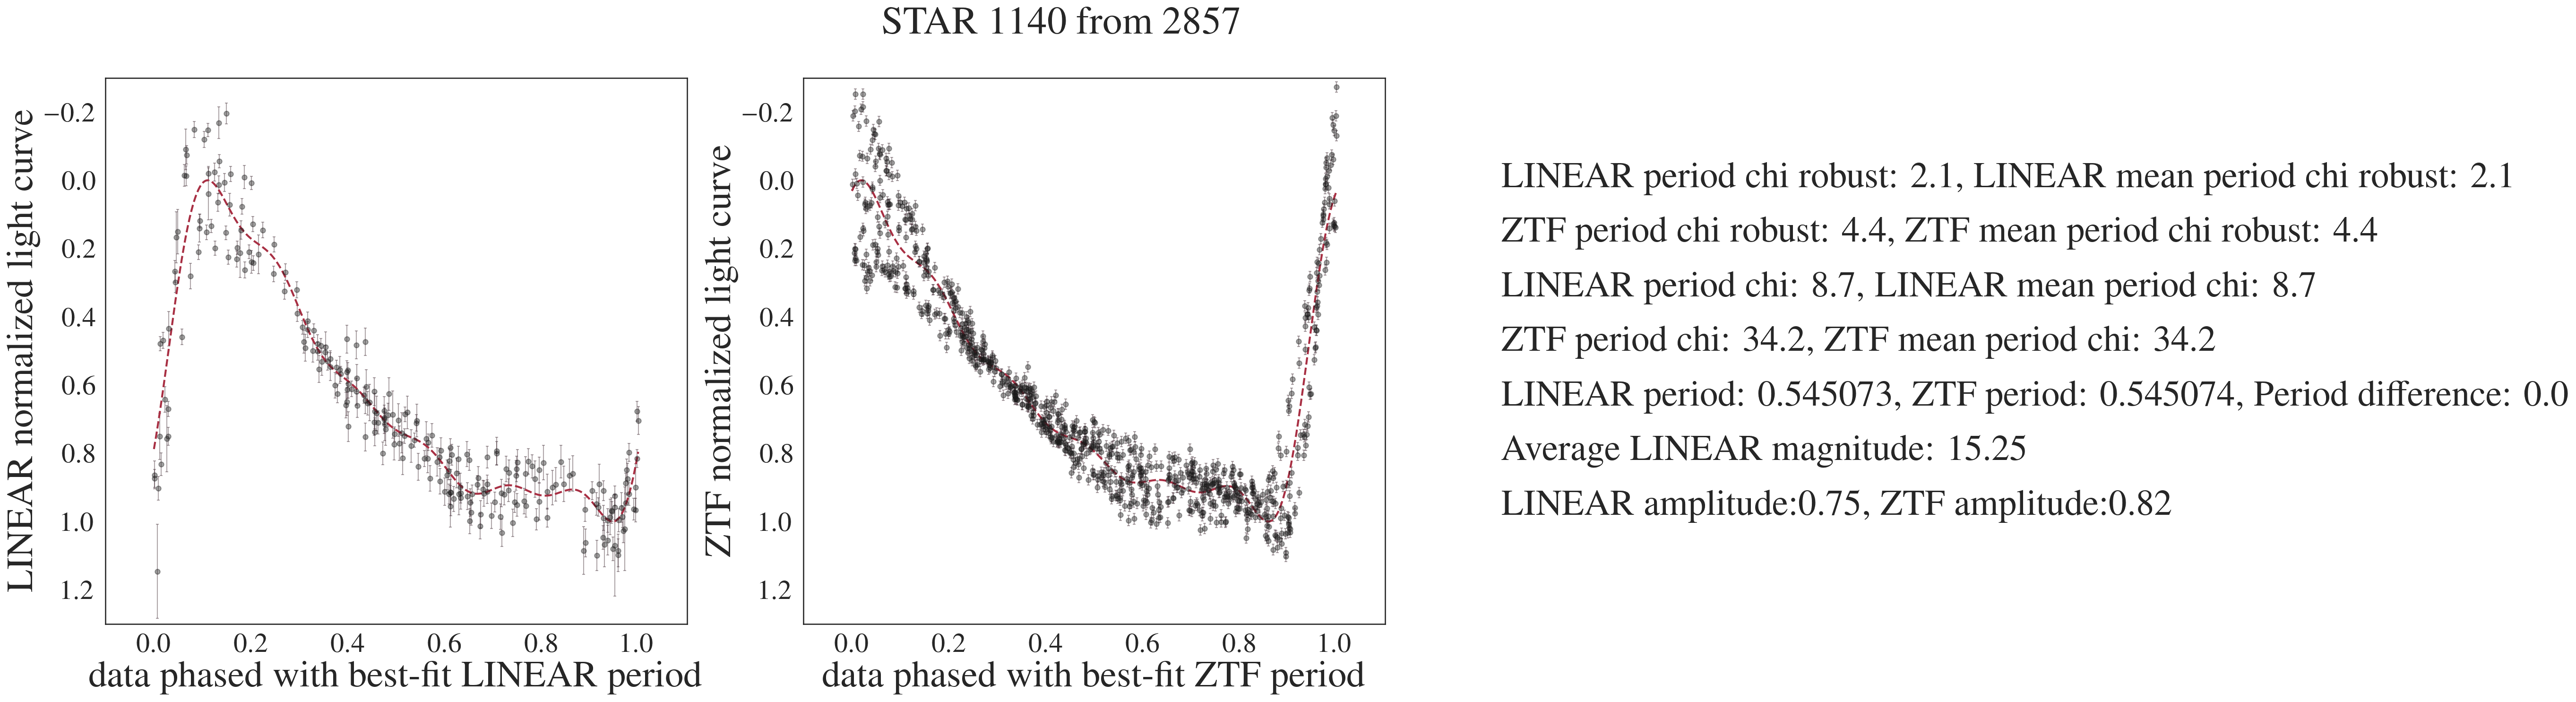
\includegraphics[width=17cm]{LCplot_10030349.png}}
  \caption{An illustration of visual analysis of phased light curves for the selected Blazhko candidates. The left
    panel shows LINEAR data and the right panel shows ZTF data
    (symbols with ``error bars'') for star with LINEARid = 1212611. The dashed
    lines are best-fit models. The numbers listed on the right side were added to aid  visual analysis. Note
    multiple coherent data point sequences offset from the best-fit mean model in the right panel.}
       \label{fig:phase1}
\end{figure*}

\begin{figure*}[ht] 
    \centering
%        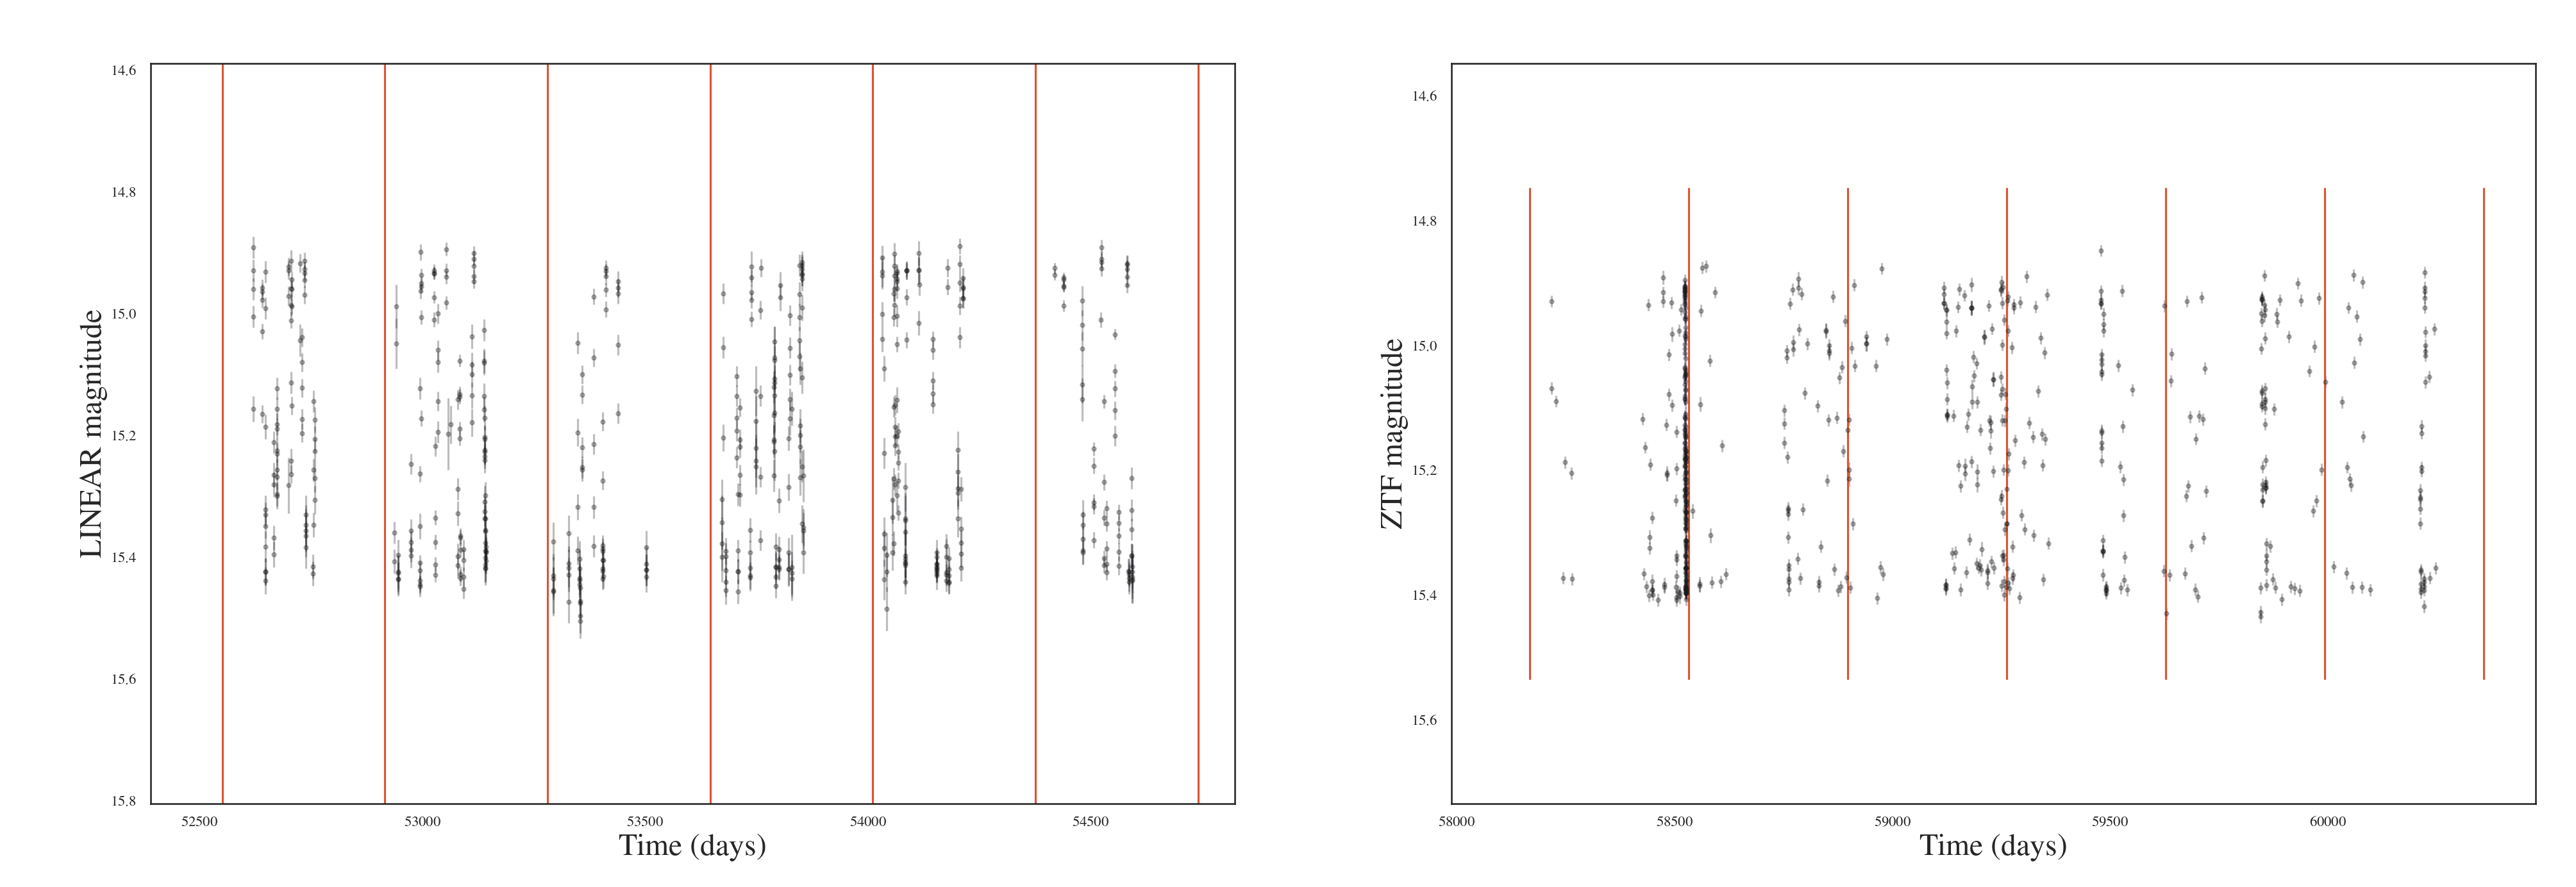
\includegraphics[width=17cm]{season_plot7048826.png}
      \resizebox{\hsize}{!}{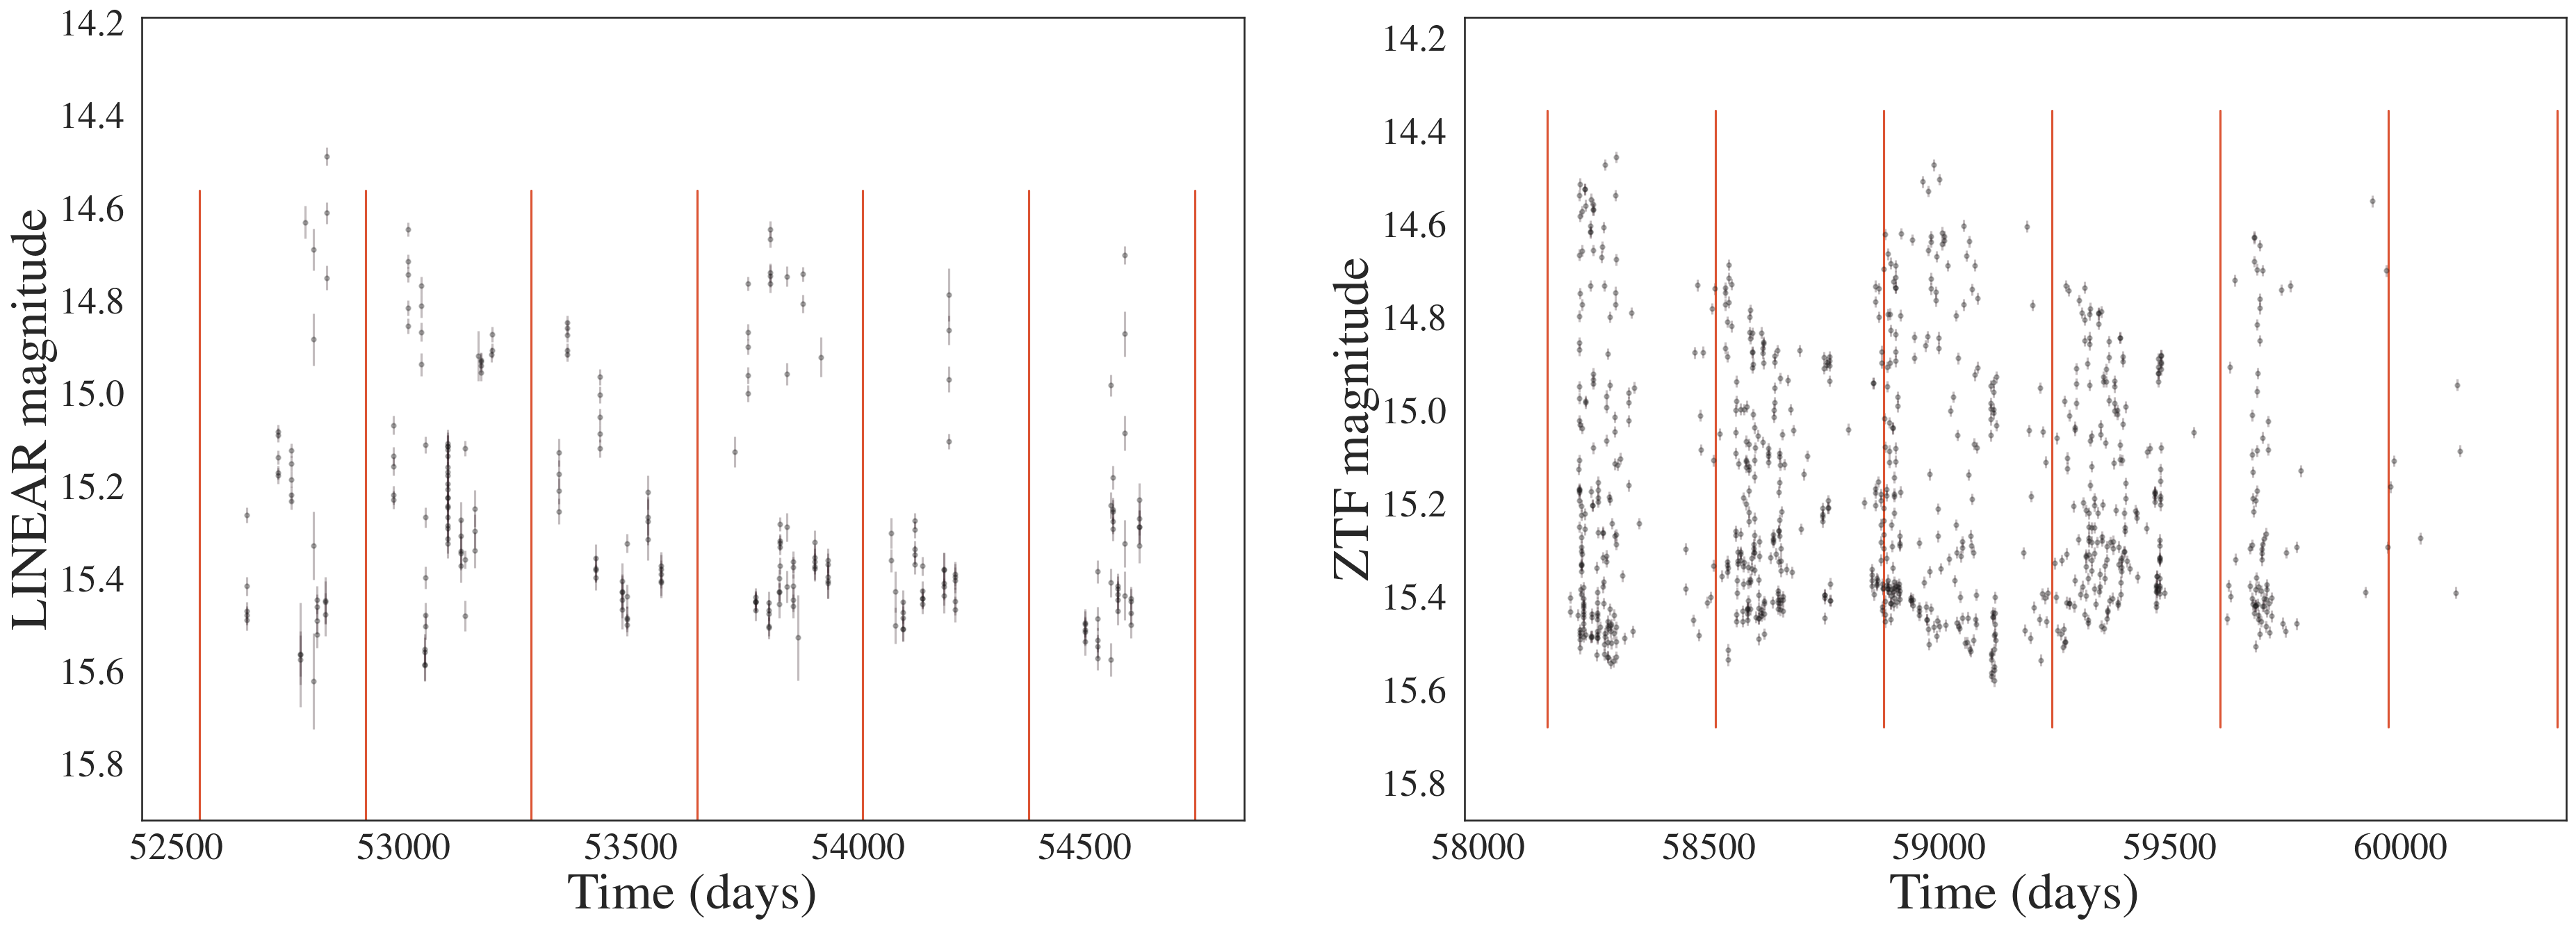
\includegraphics[width=17cm]{season_plot10030349.png}}
       \caption{An illustration of visual analysis of full light curves for the selected Blazhko candidates with emphasis
         on their repeatability between observing seasons, marked with  vertical lines (left: LINEAR data; right: ZTF data). Data
         shown are for star with LINEARid = 1212611. }
         \label{fig:phase3}
\end{figure*}
       
\begin{figure*}[ht]
    \centering
%    \includegraphics[width=17cm]{LCplotBySeason7048826.png}
    \resizebox{\hsize}{!}{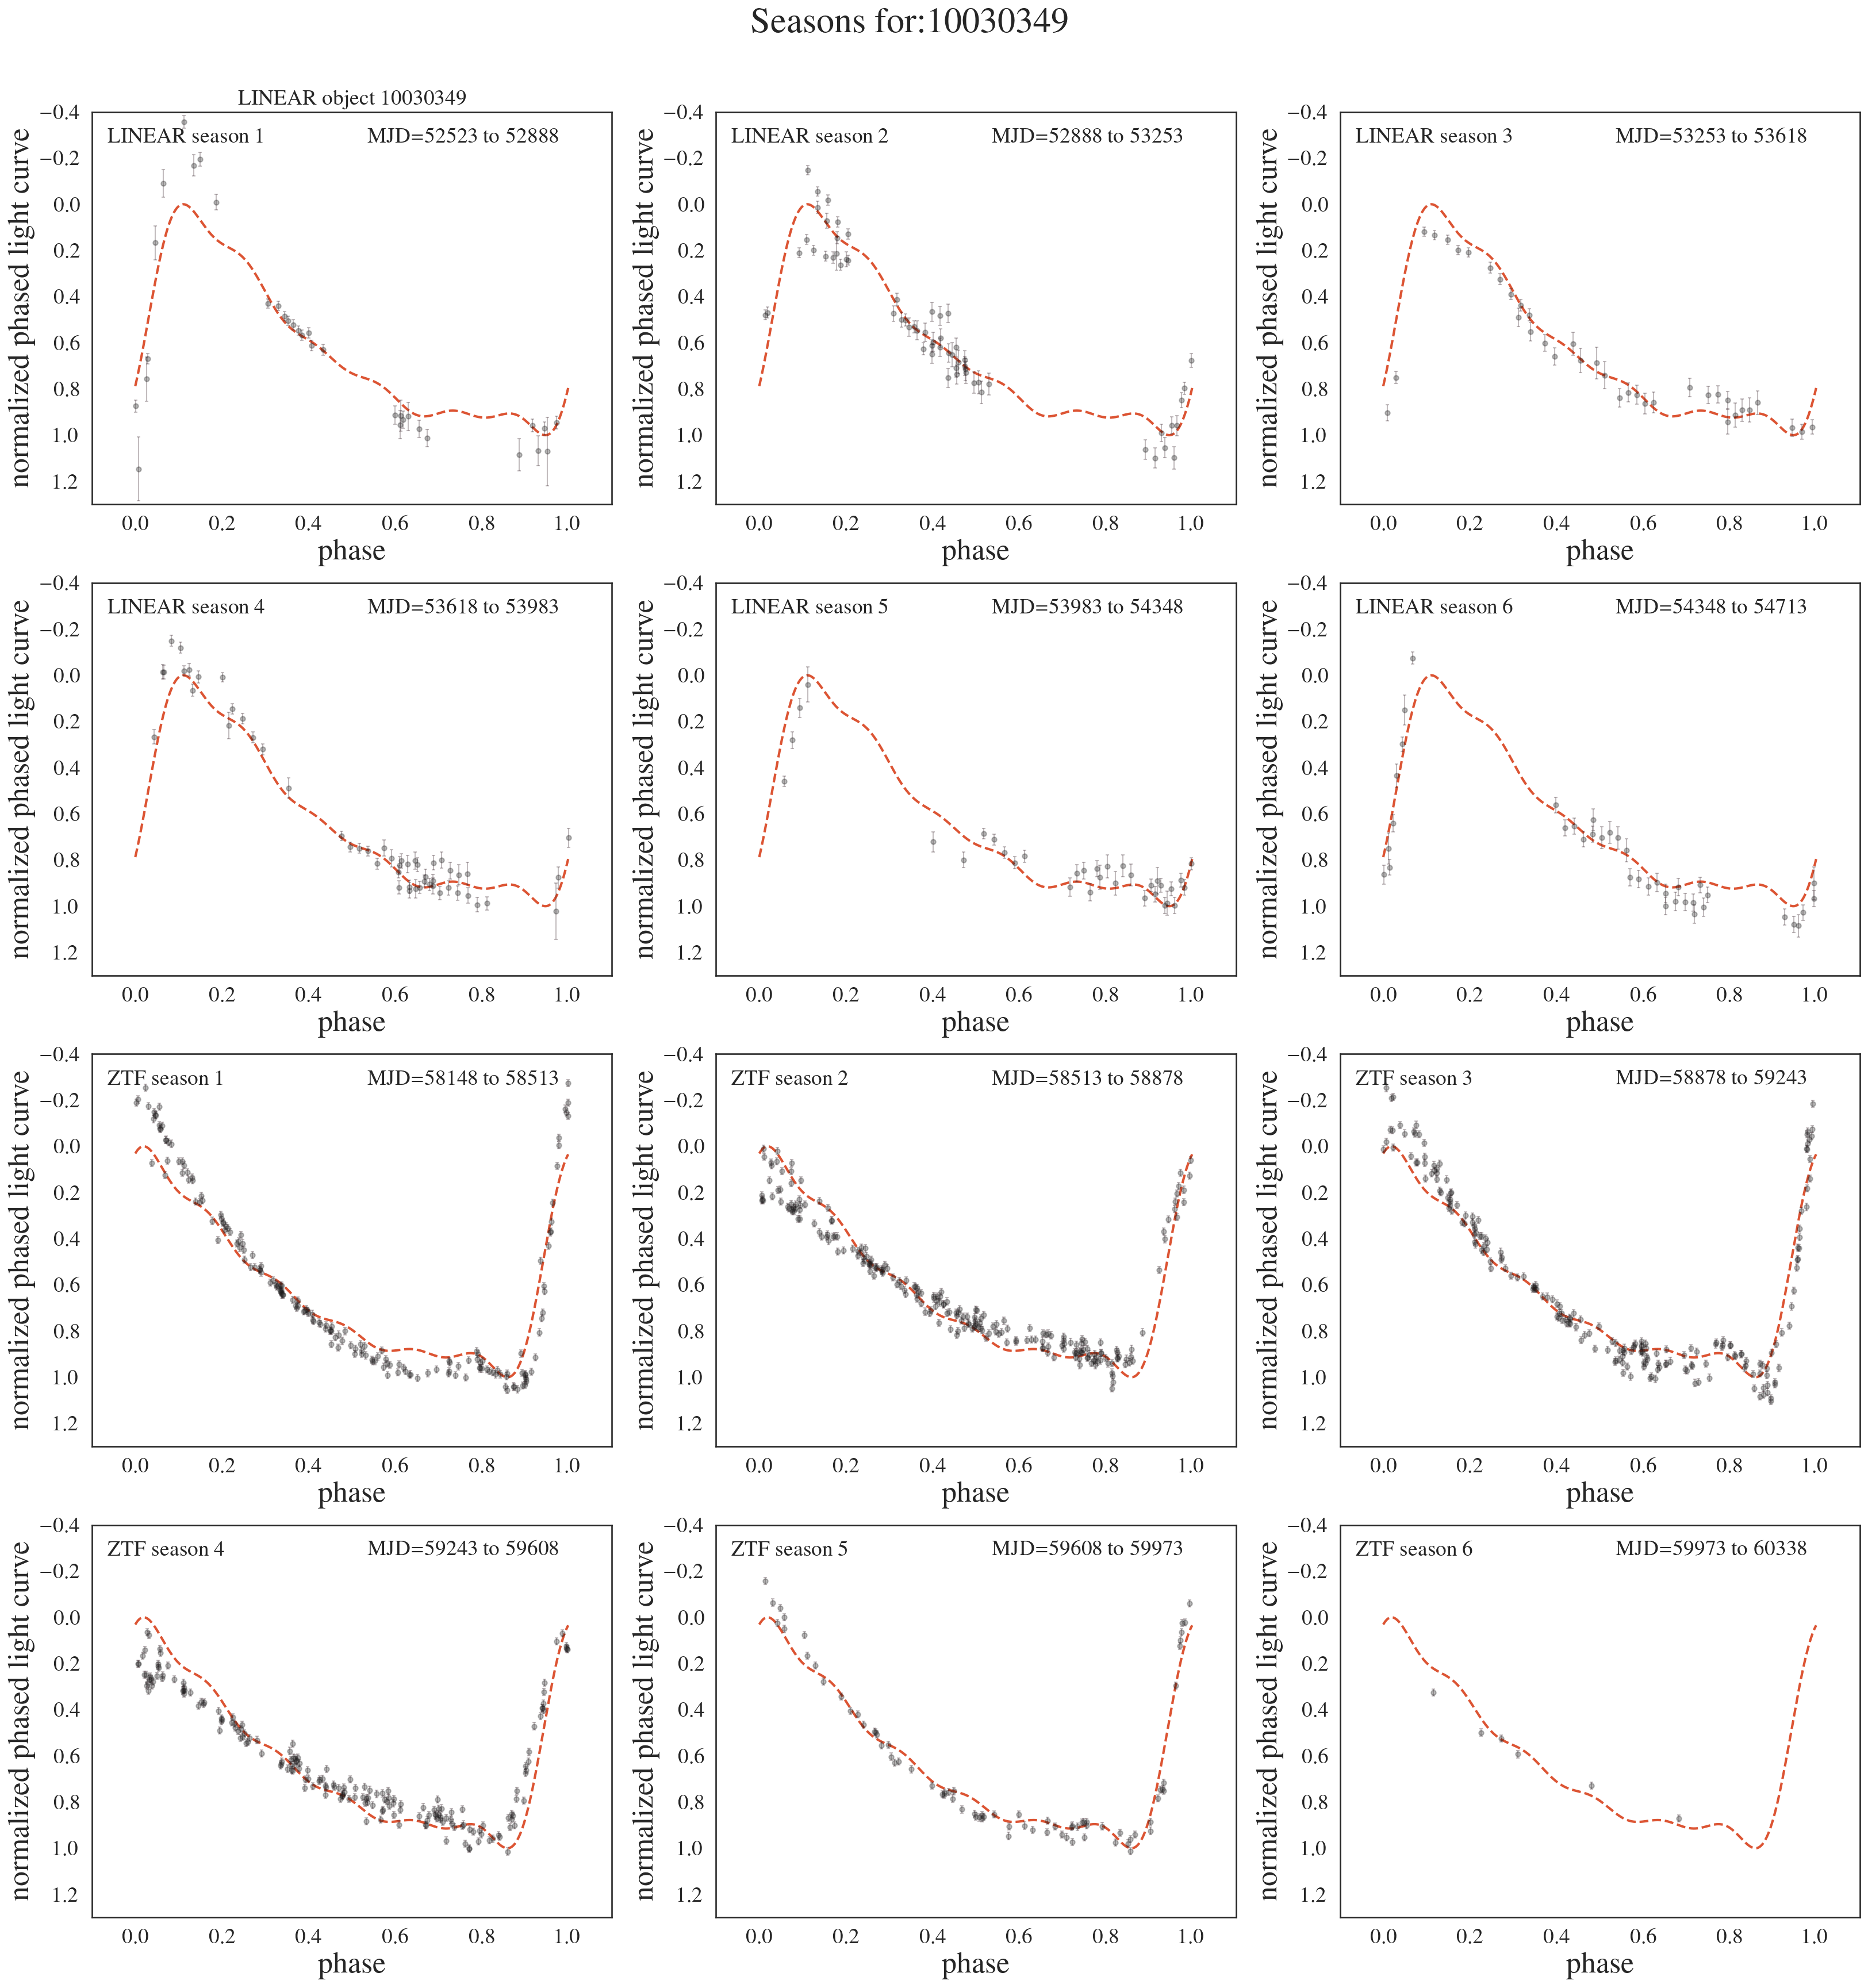
\includegraphics[width=16cm]{LCplotBySeason10030349.png}}
    \caption{The phased light curves normalized to unit amplitude are shown for single observing seasons
      and compared to the mean best-fit models (top six panels: LINEAR data; bottom six panels: ZTF data).
      Data shown are for star with LINEARid = 1212611.
      Season-to-season phase and amplitude modulations are seen in both the LINEAR and the ZTF data.}
      \label{fig:phase4}
\end{figure*}



The sample pre-selected for visual analysis includes 239 RR Lyrae stars (189 + 51, with one star selected twice),
or 8.4\% of the starting LINEAR-ZTF sample. Visual analysis included the following standard steps
\citep[e.g.,][]{2009MNRAS.400.1006J, 2017MNRAS.466.2602P}: 
\begin{enumerate}
\item The shape of the phased light curves and scatter of data points around the best-fit model were examined
    for signatures of anomalous behavior indicative of the Blazhko effect. 
    Fig.~\ref{fig:phase1} shows an example of such behavior where the ZTF data and fit show multiple coherent data point sequences
    offset from the best-fit mean model. 
  \item Full light curves were inspected for their repeatability between observing seasons (Fig.~\ref{fig:phase3}).
       This step was sensitive to amplitude modulations with periods of the order a year or longer.  
     \item The phased light curves normalized to unit amplitude were inspected for their repeatability between observing seasons.
       This step was sensitive to phase modulations of a few percent or larger on time scales of the order a year or longer.  
       Fig.~\ref{fig:phase4} shows an example of a Blazhko star where season-to-season phase (and amplitude) modulations
       are seen in both the LINEAR data and (especially) the ZTF data. 
\end{enumerate}

After visually analyzing the starting sample of 239 Blazhko candidates, we visually confirmed expected Blazhko
behavior for 136 stars (112 out of 189 and 24 out of 50). LINEAR IDs and other characteristics for confirmed
Blazhko stars are listed in Table 1 (Appendix A). Statistical properties of the selected sample of Blazhko stars are
discussed in detail in the next section. 


STOPPED HERE

